%%%%%%%%%%%%%%%%%%%%%%%%%%%%%%%%%%%%%%%%%%%%%%%%%%%%%%%%%%%%%%%%%%%%
%% I, the copyright holder of this work, release this work into the
%% public domain. This applies worldwide. In some countries this may
%% not be legally possible; if so: I grant anyone the right to use
%% this work for any purpose, without any conditions, unless such
%% conditions are required by law.
%%%%%%%%%%%%%%%%%%%%%%%%%%%%%%%%%%%%%%%%%%%%%%%%%%%%%%%%%%%%%%%%%%%%

\documentclass[
  digital,     %% The `digital` option enables the default options for the
               %% digital version of a document. Replace with `printed`
               %% to enable the default options for the printed version
               %% of a document.
%%  color,       %% Uncomment these lines (by removing the %% at the
%%               %% beginning) to use color in the printed version of your
%%               %% document
  oneside,     %% The `oneside` option enables one-sided typesetting,
               %% which is preferred if you are only going to submit a
               %% digital version of your thesis. Replace with `twoside`
               %% for double-sided typesetting if you are planning to
               %% also print your thesis. For double-sided typesetting,
               %% use at least 120 g/m² paper to prevent show-through.
  nosansbold,  %% The `nosansbold` option prevents the use of the
               %% sans-serif type face for bold text. Replace with
               %% `sansbold` to use sans-serif type face for bold text.
  nocolorbold, %% The `nocolorbold` option disables the usage of the
               %% blue color for bold text, instead using black. Replace
               %% with `colorbold` to use blue for bold text.
  lof,         %% The `lof` option prints the List of Figures. Replace
               %% with `nolof` to hide the List of Figures.
  lot,         %% The `lot` option prints the List of Tables. Replace
               %% with `nolot` to hide the List of Tables.
]{fithesis4}
%% The following section sets up the locales used in the thesis.
\usepackage[resetfonts]{cmap} %% We need to load the T2A font encoding
\usepackage[T1,T2A]{fontenc}  %% to use the Cyrillic fonts with Russian texts.
\usepackage[
  main=english, %% By using `czech` or `slovak` as the main locale
                %% instead of `english`, you can typeset the thesis
                %% in either Czech or Slovak, respectively.
  english, german, czech, slovak %% The additional keys allow
]{babel}        %% foreign texts to be typeset as follows:
%%
%%   \begin{otherlanguage}{german}  ... \end{otherlanguage}
%%   \begin{otherlanguage}{czech}   ... \end{otherlanguage}
%%   \begin{otherlanguage}{slovak}  ... \end{otherlanguage}
%%
%%
%% The following section sets up the metadata of the thesis.
\thesissetup{
    date        = \the\year/\the\month/\the\day,
    university  = mu,
    faculty     = fi,
    type        = mgr,
    department  = Department of Computer Systems and Communications,
    author      = Bc. Pavol Baran,
    gender      = m,
    advisor     = {RNDr. Lukáš Hejtmánek, Ph.D.},
    title       = {Checkpoint/Restore in Jupyterhub},
    TeXtitle    = {Checkpoint/Restore in Jupyterhub},
    keywords    = {JupyterHub, JupyterLab, Jupyter Notebook, Kubernetes, Checkpoint, Restore, Spawner},
    TeXkeywords = {JupyterHub, JupyterLab, Jupyter Notebook, Kubernetes, Checkpoint, Restore, Spawner},
    abstract    = {TODO: },
    thanks      = {I would like to thank my advisor RNDr. Lukáš Hejtmánek, Ph.D., for his help and guidance, as well as RNDr. Viktória Spišaková for helping me troubleshoot many CRIU issues. Lastly, I want to thank my family and friends for supporting me and providing an environment where I could focus on this thesis.},
    bib         = example.bib,
    %% Remove the following line to use the JVS 2018 faculty logo.
    facultyLogo = fithesis-fi,
}
\usepackage{makeidx}      %% The `makeidx` package contains
\makeindex                %% helper commands for index typesetting.
%% These additional packages are used within the document:
\usepackage{paralist} %% Compact list environments
\usepackage{amsmath}  %% Mathematics
\usepackage{amsthm}
\usepackage{amsfonts}
\usepackage{url}      %% Hyperlinks
\usepackage{markdown} %% Lightweight markup
\usepackage{listings} %% Source code highlighting
\lstset{
  basicstyle      = \ttfamily,
  identifierstyle = \color{black},
  keywordstyle    = \color{blue},
  keywordstyle    = {[2]\color{cyan}},
  keywordstyle    = {[3]\color{olive}},
  stringstyle     = \color{teal},
  commentstyle    = \itshape\color{magenta},
  breaklines      = true,
}
\usepackage{floatrow} %% Putting captions above tables
\floatsetup[table]{capposition=top}
\usepackage[babel]{csquotes} %% Context-sensitive quotation marks

%%Does \Cref links
\usepackage{hyperref}
\usepackage{cleveref}

% Only 2 leveled Contents
\addtocontents{toc}{\setcounter{tocdepth}{1}}


\begin{document}
%% The \chapter* command can be used to produce unnumbered chapters:
\chapter*{Introduction}
%% Unlike \chapter, \chapter* does not update the headings and does not
%% enter the chapter to the table of contents. I we want correct
%% headings and a table of contents entry, we must add them manually:
\markright{\textsc{Introduction}}
\addcontentsline{toc}{chapter}{Introduction}

TODO: at the end

\chapter{Project Jupyter??}
Because this thesis focuses on checkpointing and restoring Jupyter Notebooks, it is vital to understand what these notebooks are and in what scenarios they are used. This chapter describes Jupyter Notebook, its evolved iteration, Jupyter Lab, and the orchestrator of multiple running Notebooks, JupyterHub.

\section{Jupyter Notebook}
Jupyter Notebook is an open source application that allows users to easily create and share computational notebooks - documents that combine code, interactive controls, plain language, graphs, and figures, among other visualizations \cite{jupyter_notebook}.
\footnote{Note that there exist other projects focused on computation notebooks, such as the proprietary Wolfram Mathematica \url{https://www.wolfram.com/mathematica/}.}
The ability to create computational notebook comes from the fact that Jupyter Notebook runs as a web server, providing a user interface in a web browser, through which users can write code with auto-completion, execute the code, as well as provide description or annotate the code using Markdown or LaTeX languages.
On the other hand, the ability to share computational notebooks stems from simple format in which the notebooks are stored. 

The notebook documents, also commonly referred to as Jupyter Notebooks, 
\footnote{Throughout this thesis, the name \emph{Jupyter Notebook}, references only the application itself, not the notebook document that can be created through the application.}
are stored in a open document format based on JSON, and the file itself uses \emph{.ipynb} extension. The document contains complete record of the user's sessions including the output of the executed code. Since JSON is a plain text format, it allows for easy version control using Git, as well as conversion to other formats such as HTML or PDF, which can then be shared through the internet or simply, through a piece of paper \cite{jupyter_notebook}. 

\Cref{fig:jupyter-notebook-screenshot} shows the Notebooks's user interface (UI) in browser. The UI provides standard keyboard shortcuts for editing, and as already mentioned, auto-completion of code. However, apart from the functionality of word editor, the UI allows for manipulation of cells.

These cells are the main building blocks of the notebook document. There are three types of a cell \cite{jupyter_notebook}:

\begin{description}

    \item[Code cell]
    These allow for writing and executing code in a particular language, most commonly Python. The type of language depends on the \emph{Kernel} that the Jupyter Notebook server is communicating with. The exact mechanism behind the execution of code in the Notebook is out of the scope of this thesis, nevertheless there are Kernels for almost any language, with over a hundred\footnote{https://github.com/jupyter/jupyter/wiki/Jupyter-kernels} to choose from.

    \item[Markdown cell]
    These cells are meant for any text that is supposed to describe, explain, or just comment the code. Generally the text in these cells is in Markdown language, however mathematical notations can also be prescribed using LaTeX. 
    
    \item[Raw cell]
    Unlike text in Markdown cells, text in raw cell will be uninterpreted by Jupyter Notebook.
    
\end{description}


\begin{figure}[H]
  \begin{center}
  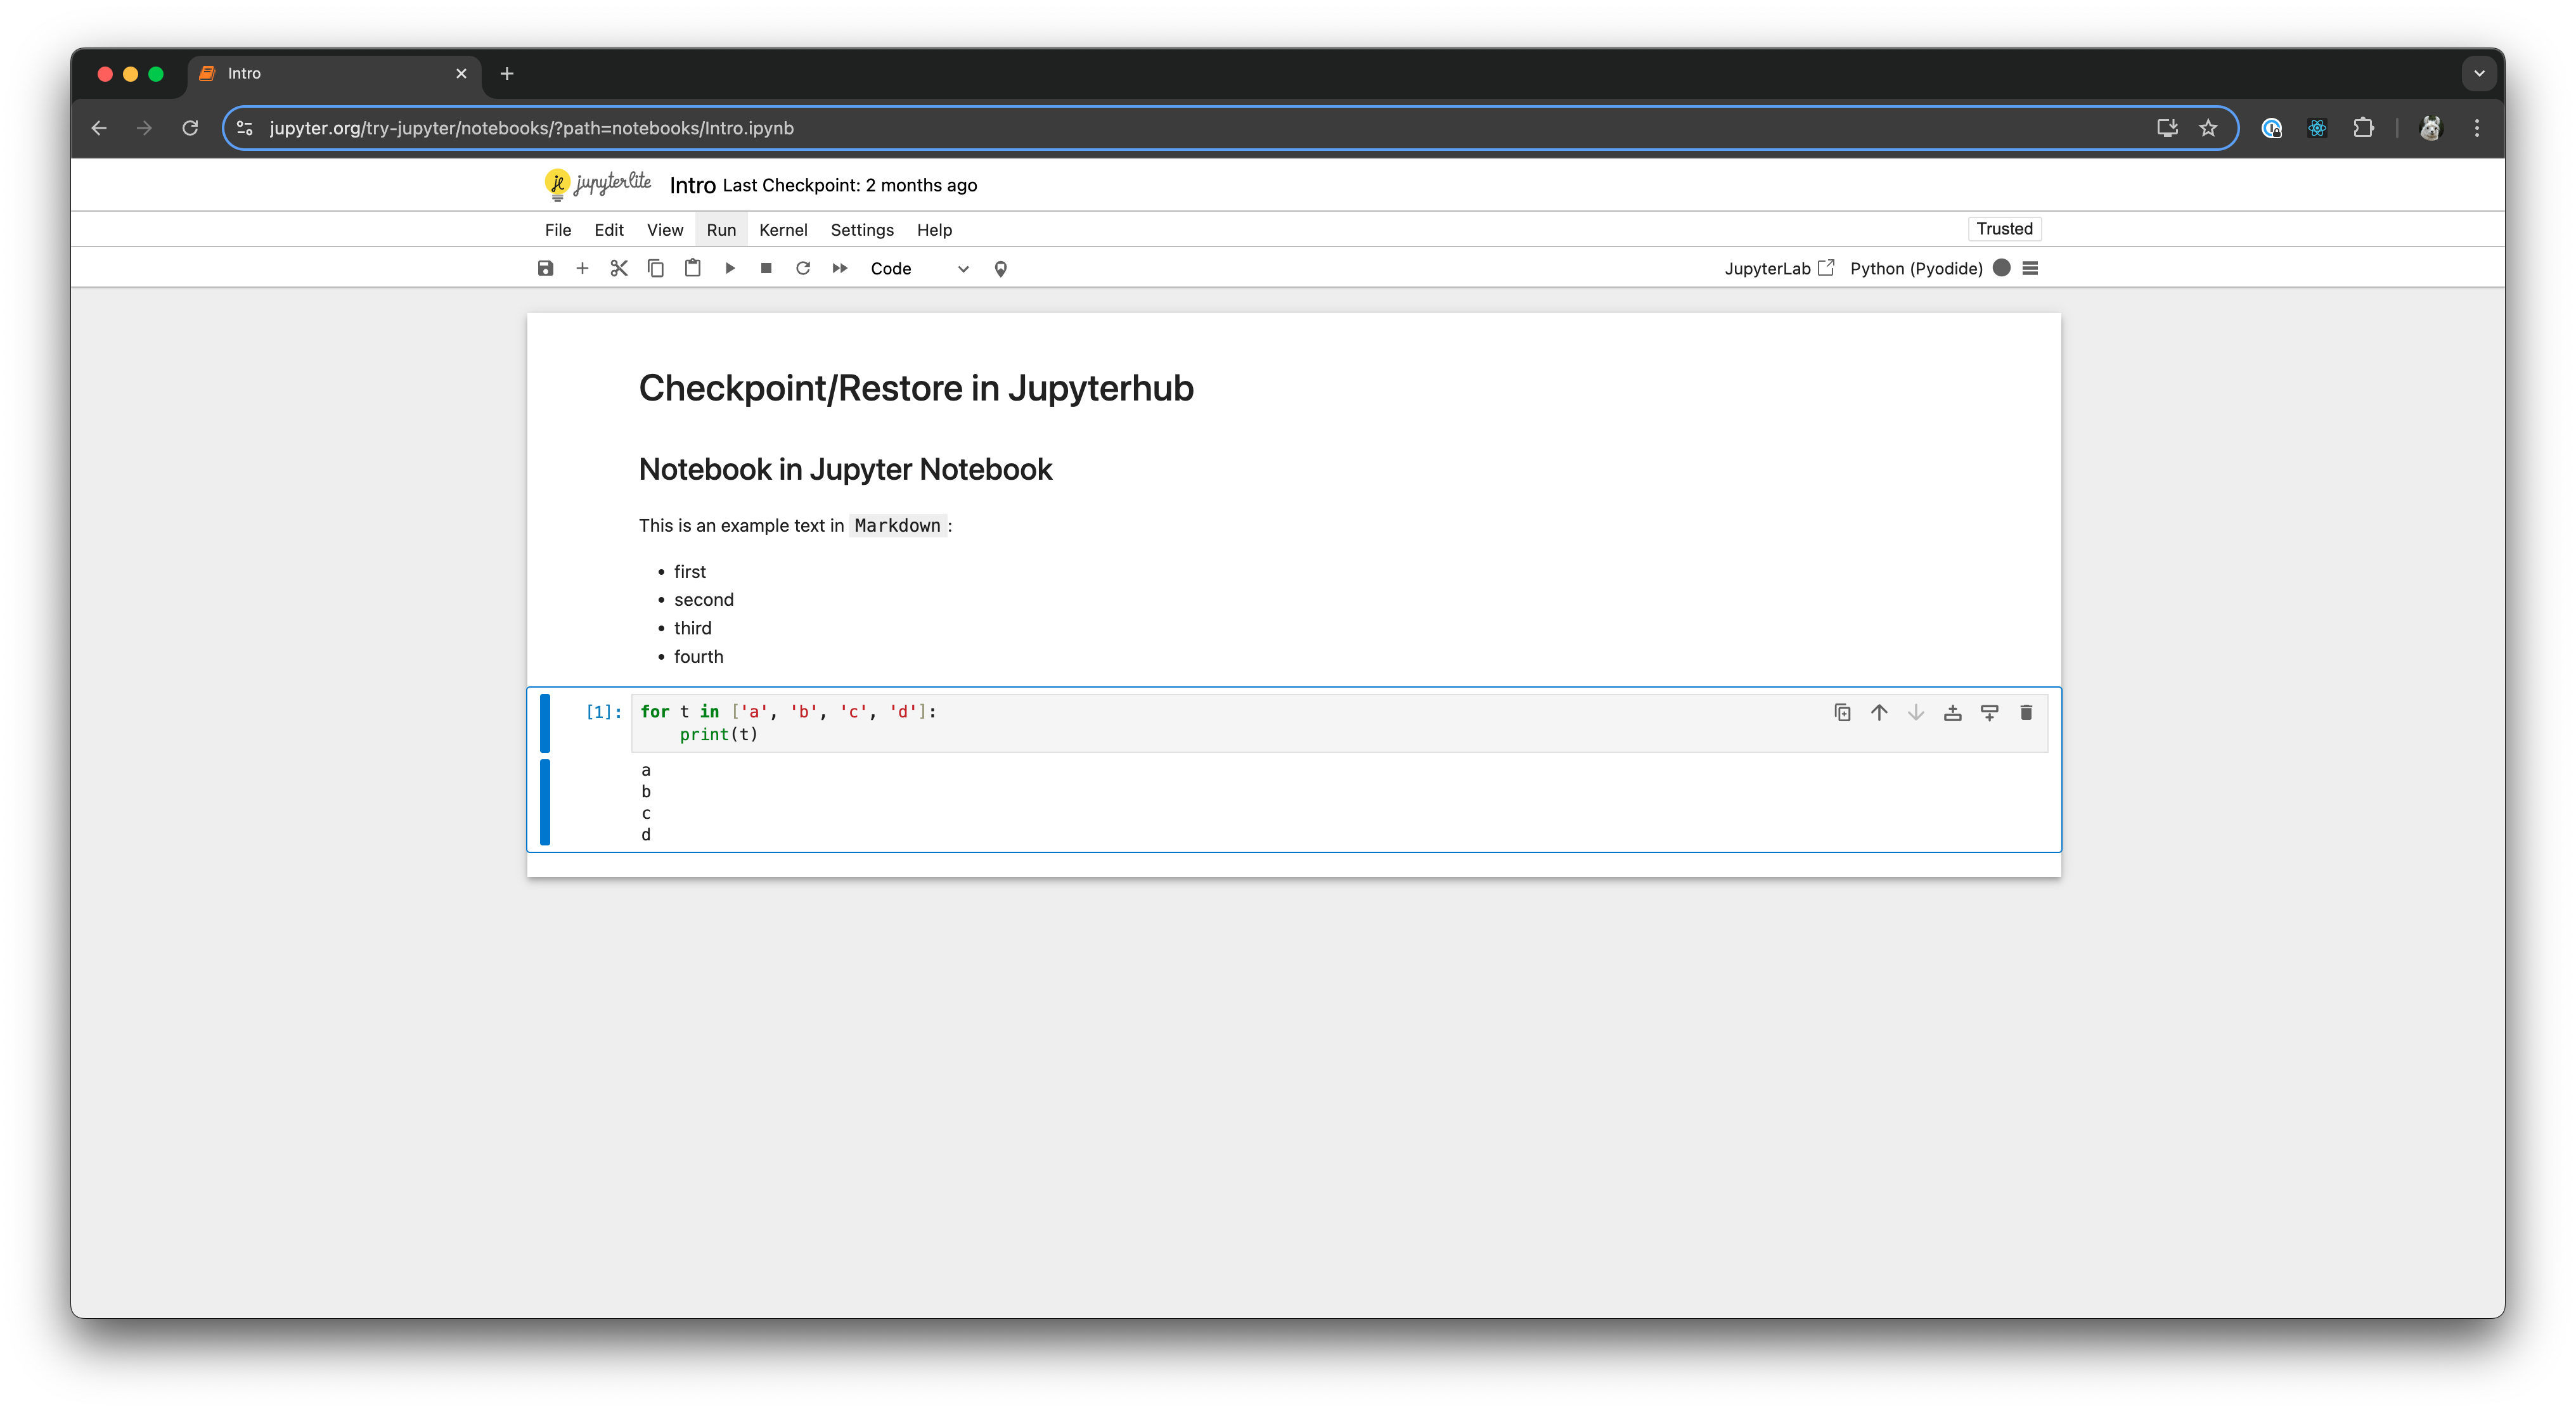
\includegraphics[width=\textwidth]{figures/jupyter-notebook-screenshot.png}
  \end{center}
  \caption{Jupyter Notebook's user interface.}
  \label{fig:jupyter-notebook-screenshot}
\end{figure}


 TODO: Jupyter Notebook has become widely used in AI research communities \url{ https://cdn.aaai.org/ocs/10349/10349-46093-1-PB.pdf} and other academical environments with over milion \url{https://ieeexplore.ieee.org/abstract/document/8816763} notebooks available online.

\section{JupyterLab}
JupyterLab's documentation describes JupyterLab as Jupyter Notebook's \emph{sibling} \cite{jupyter_lab}. However, referring to it as a sibling might give the impression that JupyterLab is merely an alternative to Jupyter Notebook. In reality, JupyterLab represents a significant advancement, offering a more sophisticated and customizable user interface which can be tailored to different use-cases. JupyterLab retains the core functionalities of Jupyter Notebook, one of which being the document format, but it expands significantly upon them by providing a modular, flexible workspace that supports multiple panels and interactive widgets as can be seen on \Cref{fig:jupyter-lab-screenshot}. Whereas Jupyter Notebook's user interface (\Cref{fig:jupyter-notebook-screenshot}) centers around one notebook document, JupyterLab resembles more of an integrated development environment (IDE), with file browser on the hand left side, and a variable inspector on the right.

\begin{figure}[H]
  \begin{center}
  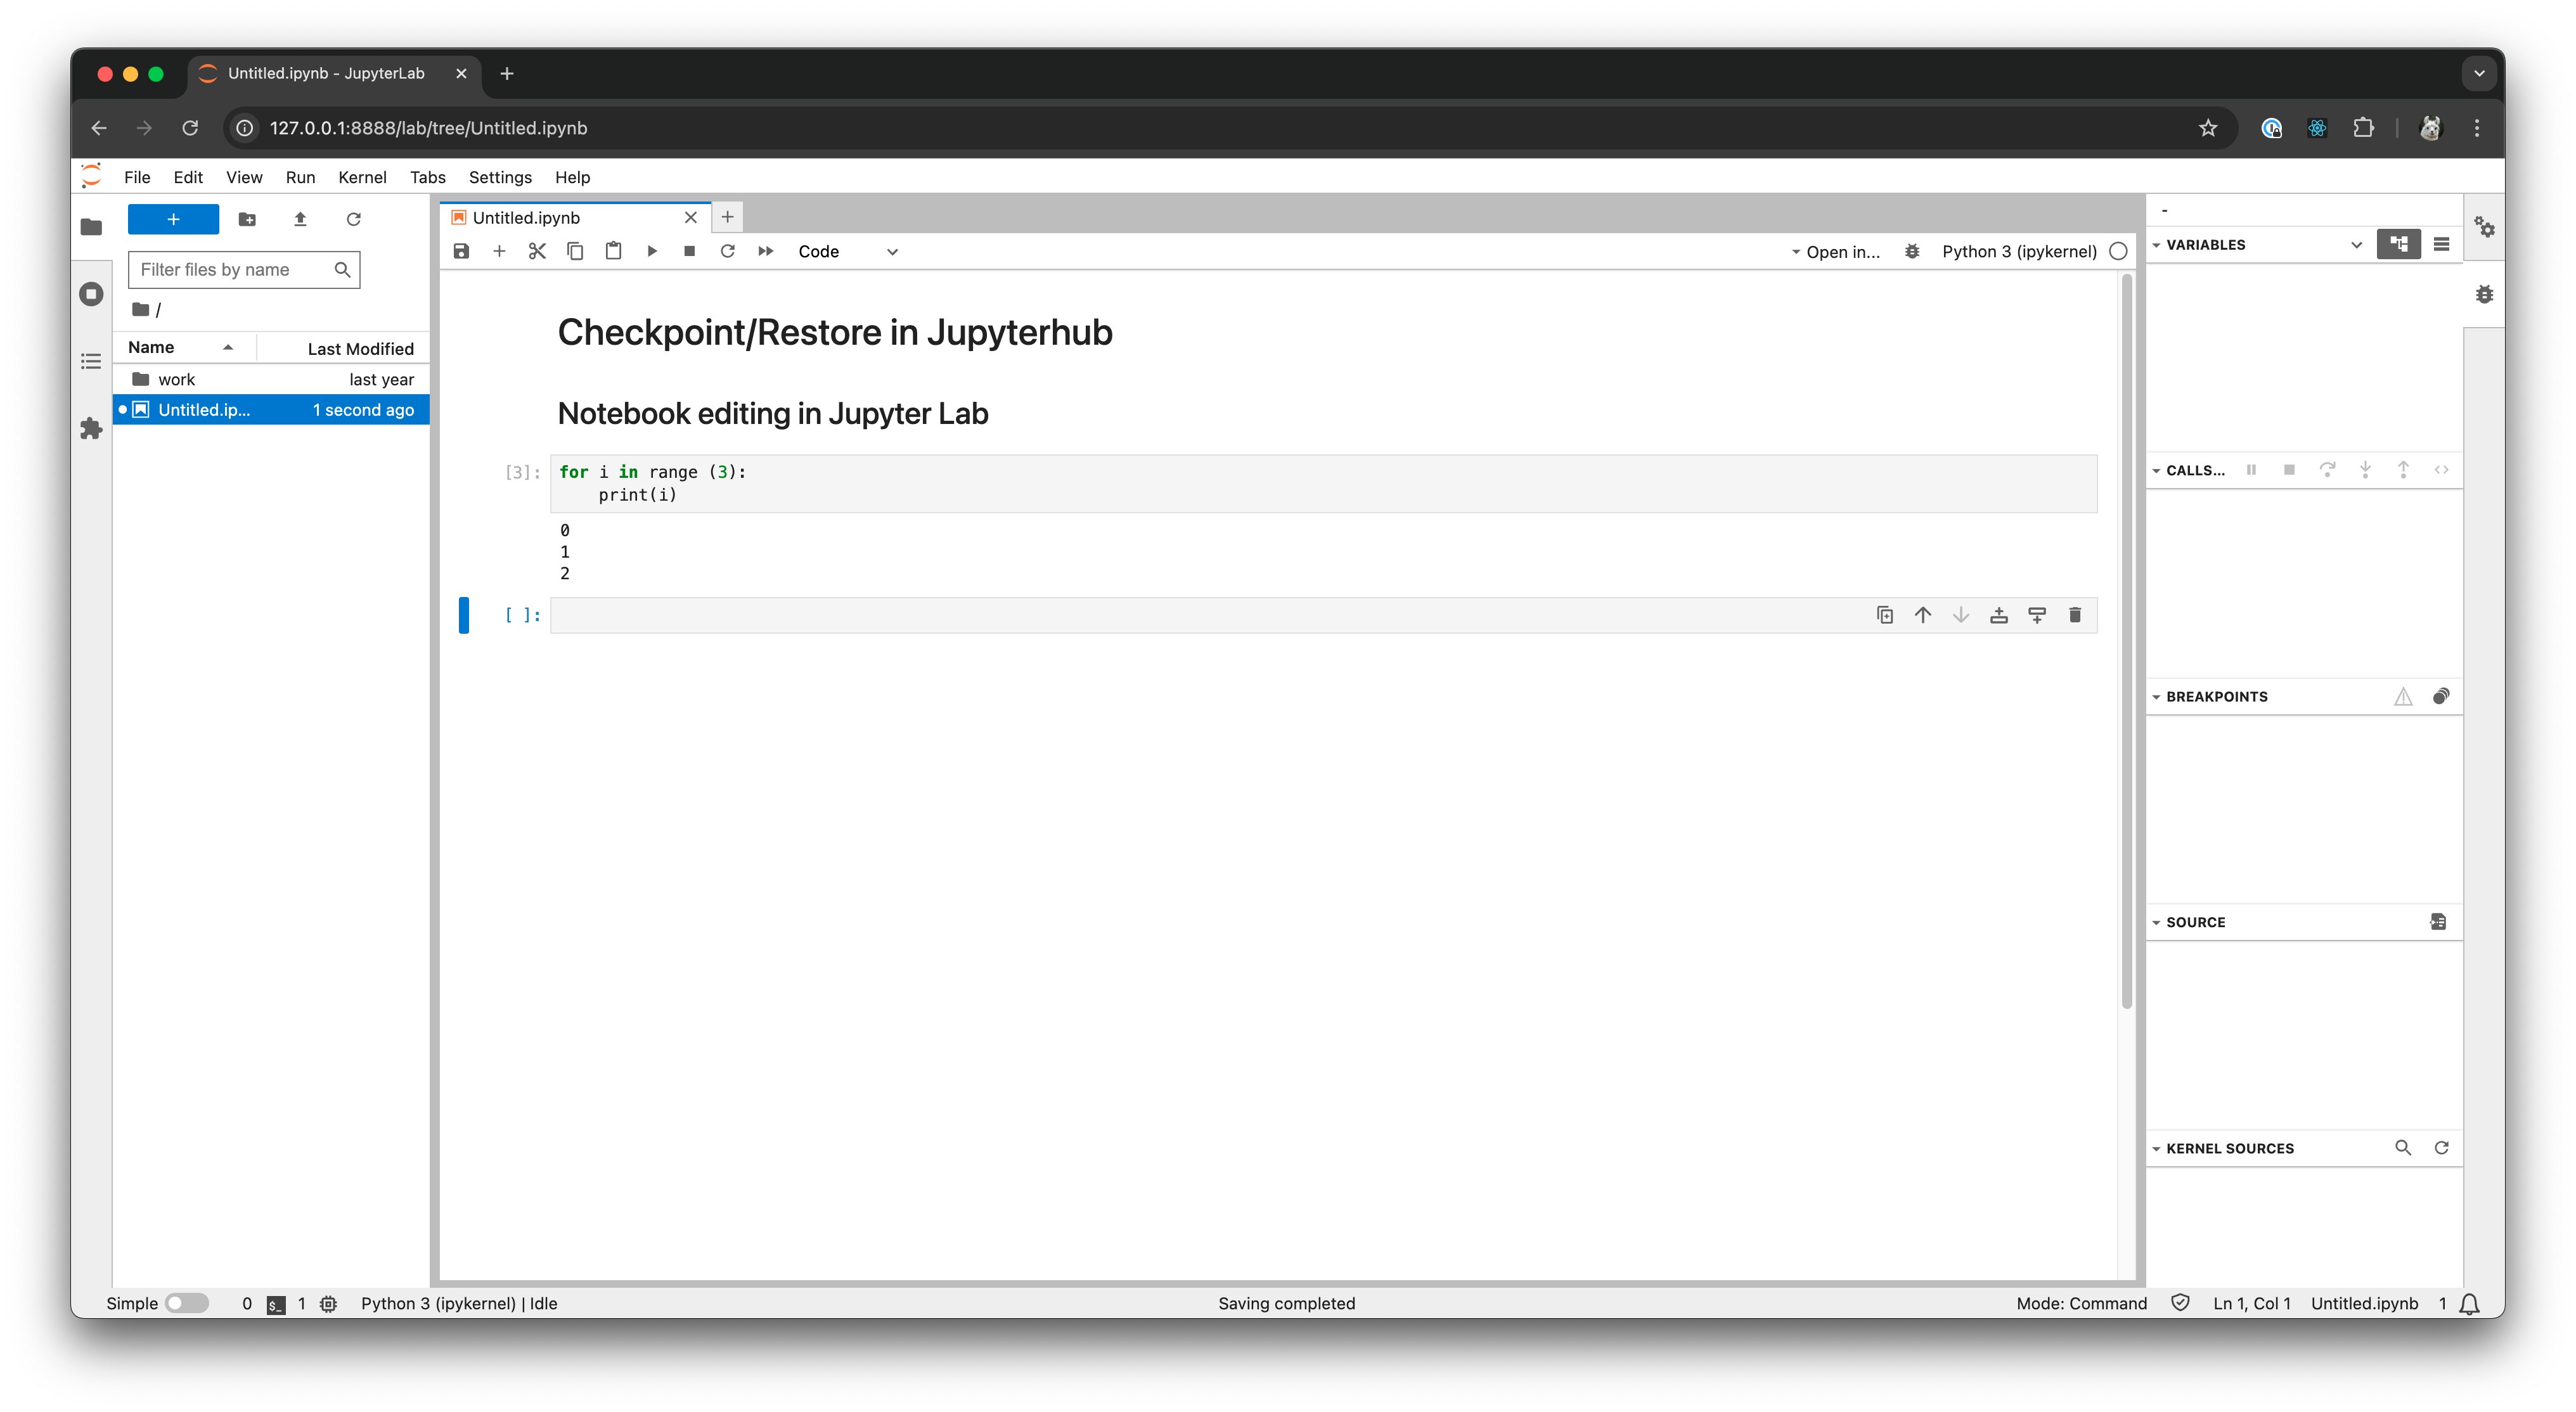
\includegraphics[width=\textwidth]{figures/jupyter-lab-extended-screenshot.png}
  \end{center}
  \caption{JupyterLab's user interface.}
  \label{fig:jupyter-lab-screenshot}
\end{figure}

All this does not negate the fact that some individuals still prefer the comparably simplified interface of Jupyter Notebook or that they do not see the value in upgrading. Moreover, as JupyterLab supports the same \emph{.ipynb} document format, and the initial versions depended on the installation of Notebook, it is not uncommon, in the community and documentation, to refer to JupyterLab as Jupyter Notebook instead. Consequently, since JupyterHub (\Cref{sec:jupyterhub}) supports both JupyterLab and Jupyter Notebook, this thesis will, henceforth, adopt the term Jupyter Notebook exclusively.

\section{JupyterHub}
\label{sec:jupyterhub}
Jupyter Notebook was initially designed for single-user environments. However, as Jupyter Notebook's popularity rose among researchers, data analyst, and academics, such did the needed for a way to quickly deploy Jupyter Notebooks for multiple users in a centralized environment, without requiring each user to install Jupyter Notebook and thus avoiding the hassle of troubleshooting installation and dependency issues.

JupyterHub addressed this need by providing a \emph{multi-user Hub that creates, manages, and proxies multiple instances of the single-user Jupyter notebook server}, which allows it to be used in \emph{a class of students, a corporate data science group, or a scientific research group} \cite{jupyterhub}. Simply put, JupyterHub takes the single-user Jupyter Notebook, and adds a layer of functionality on top, providing user management, and a control over the running environment of the Notebooks.

JupyterHub was designed with extendability in mind, and as such it comes in two main distributions \cite{jupyterhub}:

\begin{description}

    \item[The Littlest JupyterHub (TLJH)]
    Intended primarly for educators teaching small classes of ten, to at most hundred students. The distribution runs on a single server without any containerization technology such as Docker or Kubernetes and intends to provide simple as possible installation and configuration setup for JupyterHub \cite{littlest_jupyterhub}.

    \item[Zero to JupyterHub with Kubernetes (Z2JH)]
    This distribution runs in Kubernetes, with many of it's subsystems running in a separate containers, which allow it to dynamically scale up or down depending on the required resources and user demand. By utilizing several Kubernetes Nodes, the distribution is capable of serving even thousand users. This thesis builds upon the Z2JH distribution (\Cref{sec:z2jh}).
    
\end{description}

Although using one of the distributions gives some assurance of scalability, it is not the only way how to run JupyterHub. JupyterHub can be run as any Python application and configured to use specific \emph{Authenticator, Spawner, and Services} (see \Cref{subsec:jupyterhub:architecture}) based on a distinct use-case. The unofficial distribution, \emph{JupyterHub the hard way}\footnote{\url{https://github.com/jupyterhub/jupyterhub-the-hard-way/blob/master/docs/installation-guide-hard.md}}, provides a thorough walk-through for setting up JupyterHub from scratch.


\section{JupyterHub's Architecture}
\label{subsec:jupyterhub:architecture}
To give users as much freedom as possible when it comes to customizing their installation, JupyterHub is comprised of several subsystems which have multiple different implementations, enabling administrators to choose the best fit for their specific use case, such as different spawners, authenticators, and services. The following subsections provide brief look into the most important modules.


\begin{figure}[H]
  \begin{center}
  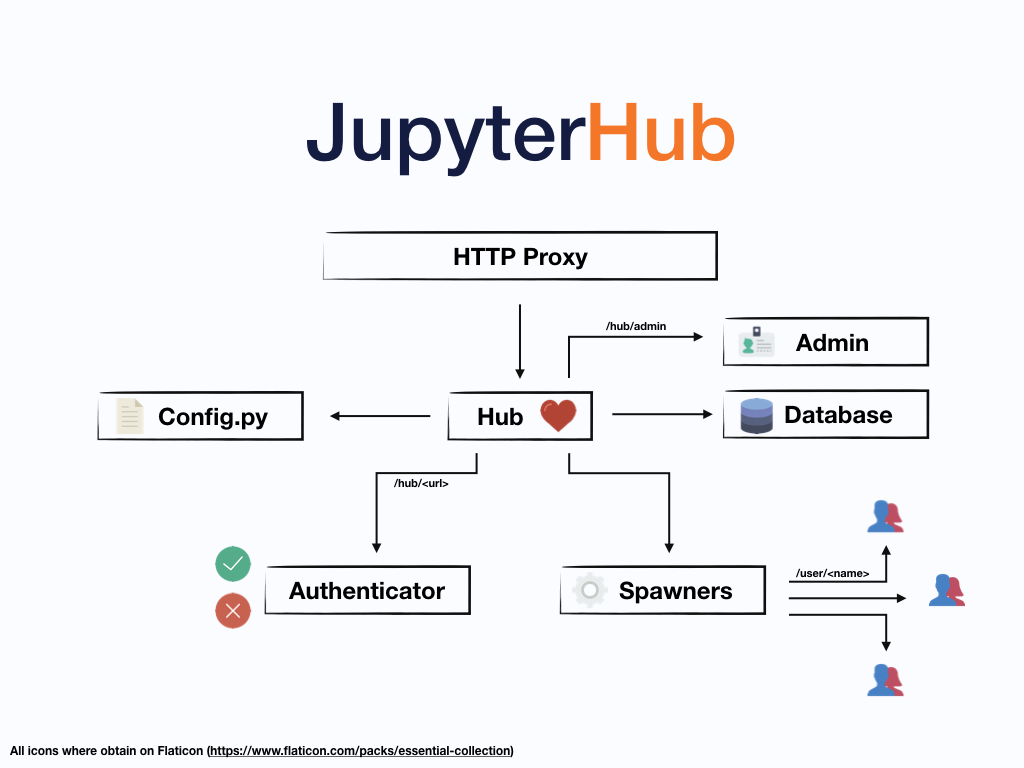
\includegraphics[width=\textwidth]{figures/jupyer-hub-architecture.jpeg}
  \end{center}
  \caption{High level architecture of JupyterHub \cite{jupyterhub}.} TODO: replace with custom diagram as this one is not representative.
  \label{fig:jupyter-hub-arch}
\end{figure}


\subsection{Configuration}
The main interface for configuration of JupyterHub is the \emph{jupyterhub\_config.py} file. 
TODO: 

\subsection{Hub}
Hub is the central piece, connecting all the modules together. Yet the end-user interacts with Hub itself only briefly, during login authentication and initialization or shutdown of Jupyter Notebooks. Hub's role is orchestrational, in that, it starts and stops the Proxy as well as Services processes, instruct Spawner when to spawn or remove Notebooks, keeps track of users, and delegates authentication of users to the Authenticator.

\subsection{Proxy}
The proxy, more specifically reverse proxy, serves as an ingress to JupyterHub. Each connection to JupyterHub and thereby to the spawned Notebooks, goes through the Proxy. 
When a user connects to JupyterHub for the first time, the Proxy forwards the connection to the Hub. Hub then delegates authentication of the user to the Authenticator, and only when the user is authenticated, instructs the Spawner to spawn the Jupyter Notebook. Once the Notebook is up and running, the Hub will update the routing table in the Proxy, to forward connections from the specific user to the spawned Notebook. Afterward, the Proxy forwards each connection of this specific user directly to the Notebook, until the user credentials expire and the whole flow is repeated, with the notable exception, that if the Notebook is already running, it does not need do be spawned.

What this basically means is that the hub itself can shut down and the proxy can continue to allow users to communicate with their notebook servers.
By default, the hub starts the proxy automatically and stops the proxy when the hub stops.
But when you configure the proxy to run separately, user’s connections will continue to work even without the hub.
(This further emphasizes that the hub is responsible for starting, not running, the notebooks)
The proxy has to be able to internally connect to both the hub and all the single-user servers.
The proxy always runs as a separate process to JupyterHub

\subsection{Authenticator}
Whenever Hub needs to authorize user's connection or request, it delegates this task to the Authenticator. The Authenticator servers as an interface between Hub and a user management system, allowing validation of user credentials and management of user accounts to be decoupled from JupyterHub. To be specific, Authenticator is a part of Hub's codebase, and as such a Python class, which can be extended to provide desired functionality.

To keep track of which Notebook belongs to which user, among other tasks, the Hub has to record information about users in a database outside the Authenticator class. Even so, the Hub stores only the data relevant to the user's role and activities in JupyterHub and does store the users themselves. The management of users, which users exist, how users login, etc., is left up to the Authenticator.


Many Authenticator implementations available delegate the user management to a third party identity provider through OAuth (OAuthenticator) or LDAP (ldapauthenticator), or the PAMAuthenticator included in JupyterHub by default, which utilizes the PAM mechanism in Linux to authenticate users. One exception to that is the NativeAuthenticator, which actually stores and validates its own usernames and passwords, effectively managing all users within JupyterHub only. The other exception is the DummyAuthenticator which allows any user to login \cite{jupyterhub_arch}.


\subsection{Spawner}
Similar to how Authenticator is an interface between Hub and the user management system, the Spawner is an interface between Hub and the running environment of Notebooks. Just like Authenticator, Spawner is a Python class in Hub's codebase and has multiple implementations depending on where how should Jupyter Notebooks be spawned. 

To define itself as Spawner, the Python class needs to be able to perform three actions \cite{jupyterhub_spawner}:

\begin{itemize}
  \item start a Jupyter Notebook
  \item poll whether a Jupyter Notebook is still running
  \item stop a Jupyter Notebook
\end{itemize}

As it should be possible for the Hub to stop without affecting the functionality, the Spawner can take advantage of two methods which allow the spawner to store it's state to the database and restore it's state from database.
TODO: \url{https://jupyterhub.readthedocs.io/en/stable/reference/api/spawner.html} load\_state get\_state

JupyterHub by default uses the LocalProcessSpawner that spawns Notebooks as local processes, however it does not work on Windows. Fortunately there are many other Spawner implementations with the notable ones being:

\begin{description}

    \item[DockerSpawner] Capable of spawning Notebooks in Docker containers on the same machine or using DockerSwarm for spawning Notebooks on remote machines \cite{jupyterhub_spawner}. The spawner can utilize Docker's API and limit the Notebook's CPU and memory usage.
    
    \item[SystemdSpawner]
    Enables to spawn Notebooks using \emph{systemd} the \emph{system and service manager} \cite{systemd} for Linux. Similarly to DockerSpawner it allows to limit the CPU and memory each Notebook is granted. \textbf{The Littlest JupyterHub} distribution uses Spawner, which is based on SystemdSpawner.

    \item[SSHSpawner]
    Can be used to spawn Notebooks on a remote server through SSH. However, the development of this Spawner seems that the project\footnote{https://github.com/NERSC/sshspawner} is no longer actively maintained.

    \item[KubeSpawner]
    Allows spawning Notebooks as Kubernetes Pods and therefore can utilize the full potential of Kubernetes API, which implies that JupyterHub must be running in Kubernetes cluster. This is the Spawner that the \textbf{Zero to JupyterHub with Kubernetes} distribution uses, and as such, this thesis is extending this Spawner with checkpoint and restore capabilities (\Cref{chap:checkpoint_spawner}).
    
\end{description}


\subsection{Services}
Services are yet another way JupyterHub can be customized or extended. In context of JupyterHub a Service is defined \emph{as something (usually a process) that can interact with the Hub’s REST API}\cite{jupyterhub_service}.

JupyterHub recognizes two types of Services. The first, \textbf{Hub-Managed Service}, are services that are started as a sub-process of Hub and managed directly by Hub. The Hub takes responsibility for starting, with a configured command and environment variables, stopping, when requested or when the Hub stops, and restarting them when they unexpectedly terminate. The second type, \textbf{Externally-Managed Services}, are independent services that are not directly controlled by the Hub but still need to interact with it. In this case, the Service does not need to be a process but might be any type of application. Both types of Services can be specified in JupyterHub's configuration file, however only Externally-Managed Services can be added or removed at runtime \cite{jupyterhub_service}.

Adding a Service to JupyterHub can have three benefits for the Service. First of all, the Service obtains an API token which it can use to call JupyterHub's REST API with configured permissions. Second benefit is that JupyterHub's Proxy can forward requests from user to the Service thus exposing the Service to the internet. Lastly, the Service can utilize the Hub's authentication mechanism to be accessible only if the user's permission allow him to.


\section{Zero to JupyterHub with Kubernetes}
\label{sec:z2jh}




\section{KubeSpawner}
\label{sec:kubespawner}




\chapter{Checkpoint/Restore in Userspace}

\section{Checkpoint/Restore in container runtimes}

\section{Checkpoint/Restore in Kubernetes}

\chapter{Checkpoint/Restore of Jupyter Notebooks in Kubernetes}

\section{Architecture}

\chapter{Checkpointer}
\label{chap:checkpointer}

\chapter{CheckpointSpawner}
\label{chap:checkpoint_spawner}


\chapter{Deployment}

\chapter{Future work}

\chapter{Conclusion}


  \printbibliography[heading=bibintoc] %% Print the bibliography.

\chapter{Inserting the index}
After using the \verb"\makeindex" macro and loading the
\texttt{makeidx} package that provides additional indexing
commands, index entries can be created by issuing the \verb"\index"
command. \index{dummy text|(}It is possible to create ranged index
entries, which will encompass a span of text.\index{dummy text|)}
To insert complex typographic material -- such as $\alpha$
\index{alpha@$\alpha$} or \TeX{} \index{TeX@\TeX} --
into the index, you need to specify a text string, which will
determine how the entry will be sorted. It is also possible to
create hierarchal entries. \index{vehicles!trucks}
\index{vehicles!speed cars}

After typesetting the document, it is necessary to generate the
index by running
\begin{center}%
  \texttt{texindy -I latex -C utf8 -L }$\langle$\textit{locale}%
  $\rangle$\texttt{ \jobname.idx}
\end{center}
from the command line, where $\langle$\textit{locale}$\rangle$
corresponds to the main locale of your thesis -- such as
\texttt{english}, and then typesetting the document again.

The \texttt{texindy} command needs to be executed from within the
directory, where the \LaTeX\ source file is located. In Windows,
the command line can be opened in a directory by holding down the
\textsf{Shift} key and by clicking the right mouse button while
hovering the cursor over a directory. Select the \textsf{Open Command
Window Here} option in the context menu that opens shortly
afterwards.

With online services -- such as Overleaf -- the commands are
executed automatically, although the locale may be erroneously
detected, or the \texttt{makeindex} tool (which is only able to
sort entries that contain digits and letters of the English
alphabet) may be used instead of \texttt{texindy}. In either case,
the index will be ill-sorted.

  \makeatletter\thesis@blocks@clear\makeatother
  \phantomsection %% Print the index and insert it into the
  \addcontentsline{toc}{chapter}{\indexname} %% table of contents.
  \printindex


\appendix %% Start the appendices.
\chapter{An appendix}
Here you can insert the appendices of your thesis.

\end{document}
